\documentclass{beamer}

\usepackage[utf8]{inputenc}
\usepackage[T1]{fontenc}
\usepackage[francais]{babel}
\usetheme{Warsaw}

\title{Stage de 5\ieme année}
\subtitle{Éco-conception de logiciel}
\author{Guillaume Delamare}
\institute{EMN - Équipe ASCOLA}
\date{\today}

\AtBeginSection[]
{
  \begin{frame}<beamer>
    \frametitle{Plan}
    \tableofcontents[currentsection, hideallsubsections]
  \end{frame}
}

\begin{document}
    \begin{frame}
	\titlepage
    \end{frame}

    \section*{Introduction}
	\begin{frame}
	    \frametitle{Plan}
	    \tableofcontents[hideallsubsections]{}
	\end{frame}
	
    \section{Présentation du sujet de stage}
	\begin{frame}{Contexte}
	    \begin{itemize}
		\item Travaux GreenIT de l'équipe ASCOLA
		\item D'autres projets - Code Vert (Projet labélisé par le pôle de compétitivité Images et Réseaux)
		\item Des sociétés intéressées - SIGMA - Additeam
	    \end{itemize}
	\end{frame}
    	\begin{frame}{Sujet}
	    \begin{itemize}
		\item Forte augmentation des équipements informatique de par le monde
		\item La consommation d'énergie des système d'information un enjeu pour le futur
		\item Plusieurs travaux sur la consommation du matériel
		\item Peu de travaux sur la consommation de la couche logicielle
	    \end{itemize}
	\end{frame}
	\begin{frame}{Objectifs}
	    Définir des techniques, des patterns et des outils pour rendre moins énergivore les logiciels
	    \begin{block}{Pour cela, il faut :}
	    \begin{itemize}
		\item Identifier les travaux réalisés dans le domaine
		\item Mettre au point une méthodologie permettant de quantifier l'énergie consommée
		\item Faire des propositions et les expérimenter
	    \end{itemize}
	    \end{block}
	\end{frame}
		
    \section{Mesure de la consommation}
	\begin{frame}{Outils de mesure de la consommation}
	    \begin{block}{Liste des outils testés}
		\begin{itemize}
		    \item pTop
		    \item Energy Checker
		    \item ClassMexer
			\item Wattsup Pro
		    \item JouleMeter
		    \item PowerAPI
		\end{itemize}
	    \end{block}	
	\end{frame}
	\begin{frame}{Outils de mesure de la consommation}
		\begin{block}{Problème rencontré}
			Aucun de ces outils ne permet de mesurer réellement et suffisament la consommation énergétique d'un logiciel.
		\end{block}
		Il faut donc croiser les résultats des outils disponibles.
	\end{frame}
	
    \section{Bonnes pratiques de programmation}
	\begin{frame}{Exemple de bonnes pratiques}
    	    \begin{block}{En java}
		Utiliser un StringBuffer pour manipuler une chaine de caractères plutôt qu'un String.
	    \end{block}
    	    \begin{block}{En C}
		Faire attention à l'ordre des déclarations dans une structure.
	    \end{block}
	\end{frame}
	
    \section{Architecture logicielle}
	\begin{frame}{Modularité du code}
	    \begin{block}{OSGi}
		\begin{itemize}
		    \item Une spécification écrite par l'OSGi Alliance
		    \item Différentes inplémentations (Felix, Equinox, Knopflerfish...)
		    \item Un système permettant de construire des applications modulaires
		\end{itemize}
	    \end{block}
	\end{frame}
	\begin{frame}{Modularité du code}
	Une application qui charge et décharge des modules en fonction de ces besoins.
	    \begin{center}
		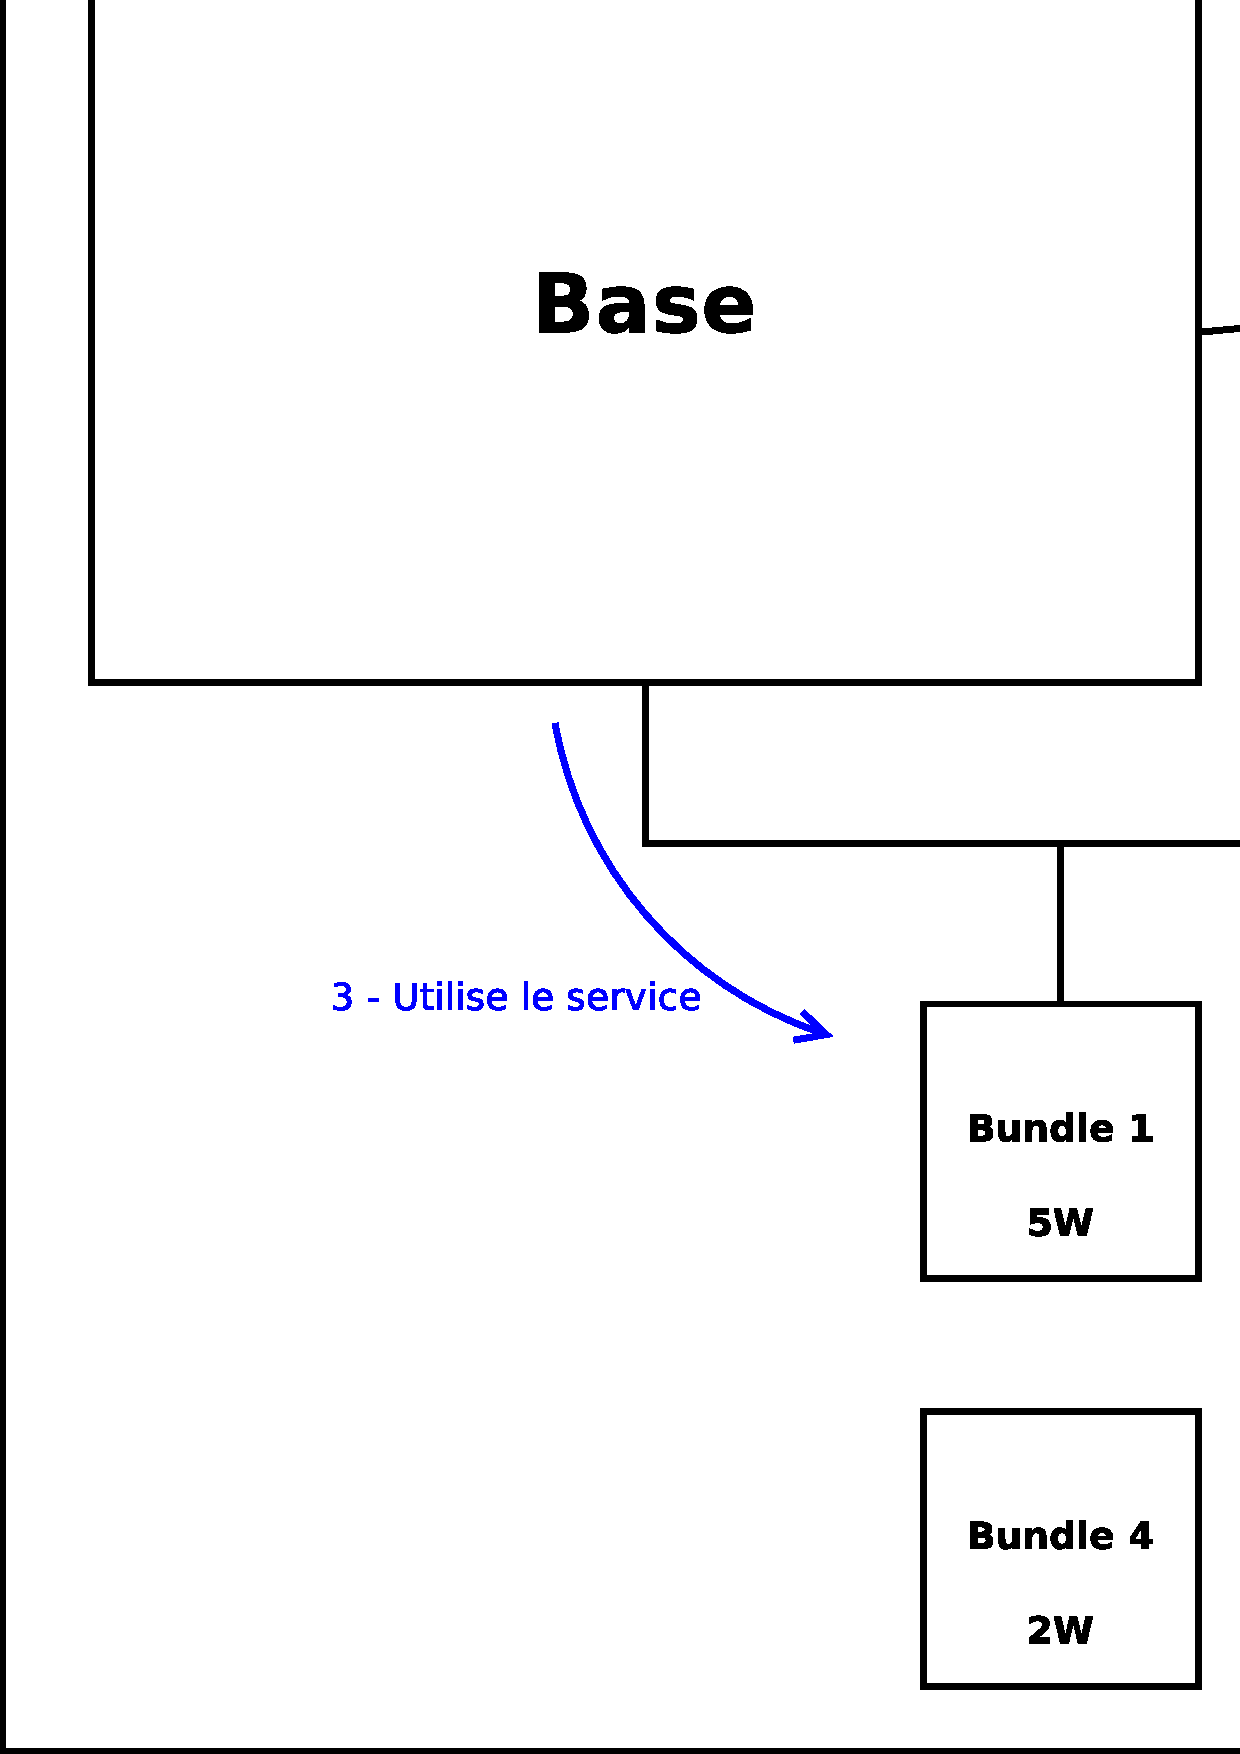
\includegraphics[width=200px]{../../Figures/OSGi/EcoPattern_General_Figure.png}
	    \end{center}
	\end{frame}
	
    \section{Bilan et Plan de route}
	\begin{frame}{Bilan et Plan de route}
		\begin{block}{Bilan}
		\begin{itemize}
			\item De gros problèmes rencontrés sur la mesure de consommation
			\item Un sujet très vaste mais de premiers résultats encourageants
		\end{itemize}
		\end{block}
		\begin{block}{Et pour la suite ?}
		\begin{itemize}
			\item Implémenter le prototype d'application modulaire
			\item Finir le développement de l'application de tri
			\item Synthétiser les résultats obtenus
		\end{itemize}
		\end{block}
	\end{frame}

    \section*{Questions}
	\begin{frame}{Questions}
	    \begin{columns}[c]
		\begin{column}{5cm}
		    Avez vous des questions ?
		\end{column}
    		\begin{column}{5cm}
    		    \begin{figure}
			%\includegraphics[width=6cm]{diagramme/}
		    \end{figure}
		\end{column}
	    \end{columns}
	\end{frame}
\end{document}
